\documentclass[12pt,a4paper]{scrartcl}
\usepackage[utf8]{inputenc}
\usepackage{siunitx}
\usepackage{graphicx}
\usepackage{amsmath}
\usepackage{float}
\usepackage{pdfpages}
\usepackage{circuitikz}

\newcommand{\n}[1]{\mkern 1.5mu\overline{\mkern-1.5mu#1\mkern-1.5mu}\mkern 1.5mu}
\newcommand{\g}[1]{\\\stackrel{\text{#1}}{=}}

\begin{document}
	\title{Grundlagen der Rechnerarchitektur\\ Übungsblatt 8}
	\date{}
	\author{Tarik Enderes, Jonas Strauch}
	\maketitle
	
	\begin{description}
		\item[1.] 
		\begin{description}
			\item[a)] 
			\begin{tabular}{c c c | c c c c c c c c}
				$x_2$ & $x_1$ & $x_0$ & $y_7$ & $y_6$ & $y_5$ & $y_4$
				& $y_3$ & $y_2$ & $y_1$ & $y_0$\\\hline
				0 & 0 & 0 & 0 & 0 & 0 & 0 & 0 & 0 & 0 & 1\\
				0 & 0 & 1 & 0 & 0 & 0 & 0 & 0 & 0 & 1 & 0\\
				0 & 1 & 0 & 0 & 0 & 0 & 0 & 0 & 1 & 0 & 0\\
				0 & 1 & 1 & 0 & 0 & 0 & 0 & 1 & 0 & 0 & 0\\
				1 & 0 & 0 & 0 & 0 & 0 & 1 & 0 & 0 & 0 & 0\\
				1 & 0 & 1 & 0 & 0 & 1 & 0 & 0 & 0 & 0 & 0\\
				1 & 1 & 0 & 0 & 1 & 0 & 0 & 0 & 0 & 0 & 0\\
				1 & 1 & 1 & 1 & 0 & 0 & 0 & 0 & 0 & 0 & 0\\
			\end{tabular}
		\item[b)]
		\begin{math}
		y_0 = \n{x_0}\n{x_1}\n{x_2} = \n{x_0+x_1+x_2}\\
		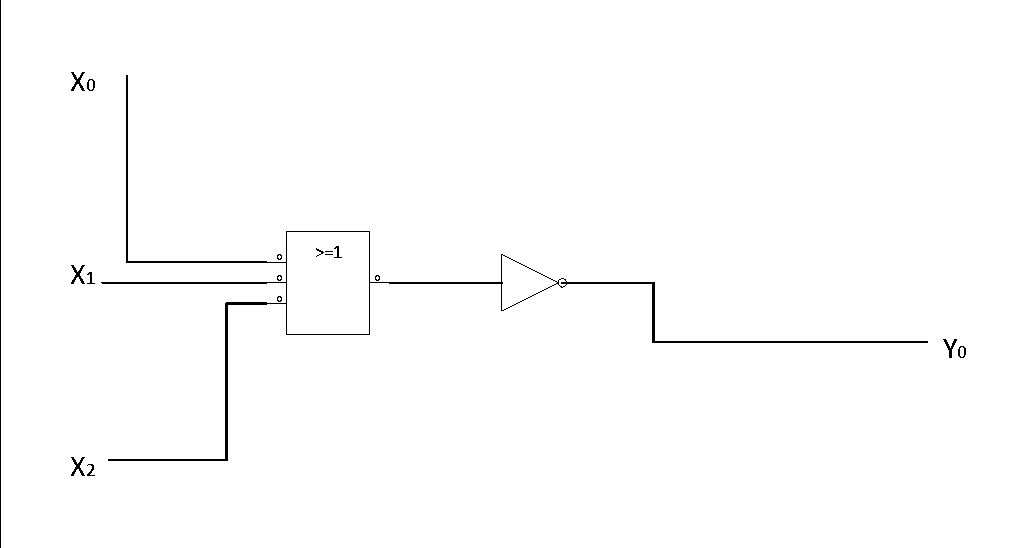
\includegraphics[width=10cm]{y0}\\
		y_1 = x_0\n{x_1}\n{x_2} = x_0 \cdot \n{x_1+x_2}\\
		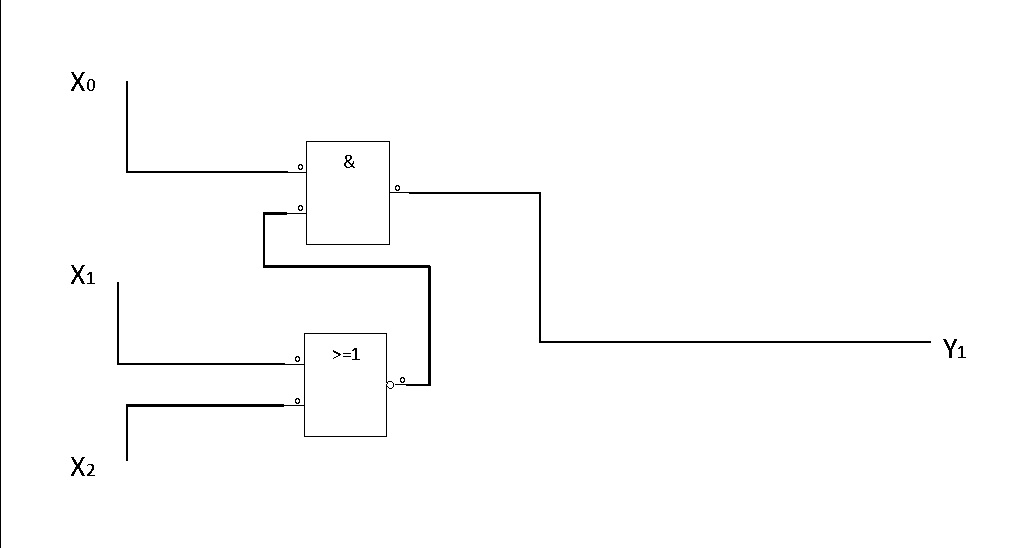
\includegraphics[width=10cm]{y1}\\
		y_2 = \n{x_0}x_1\n{x_2} = x_1 \cdot \n{x_0+x_2}\\
		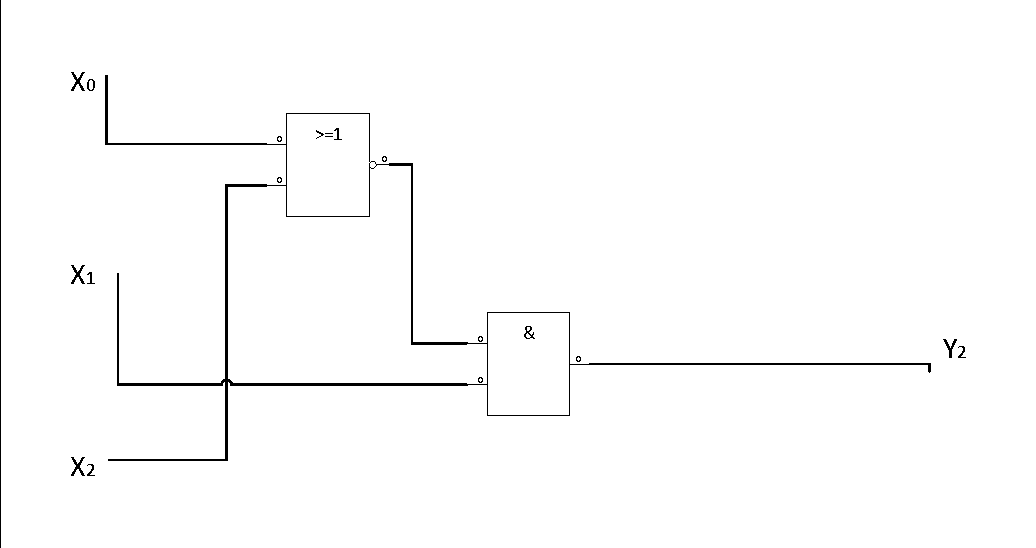
\includegraphics[width=10cm]{y2}\\
		y_3 = x_0x_1\n{x_2}\\
		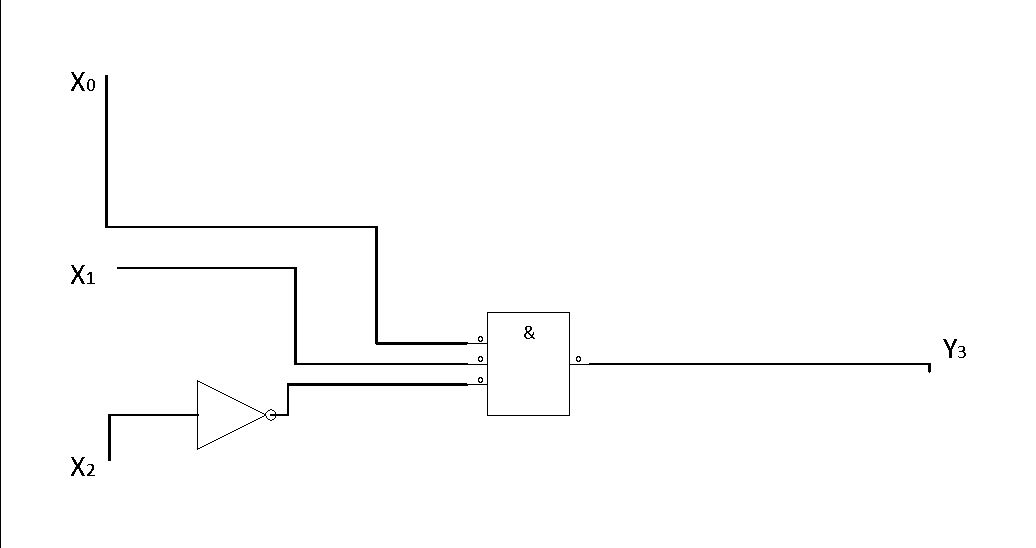
\includegraphics[width=10cm]{y3}\\
		y_4 = \n{x_0}\n{x_1}x_2 = x_2 \cdot \n{x_0+x_1}\\
		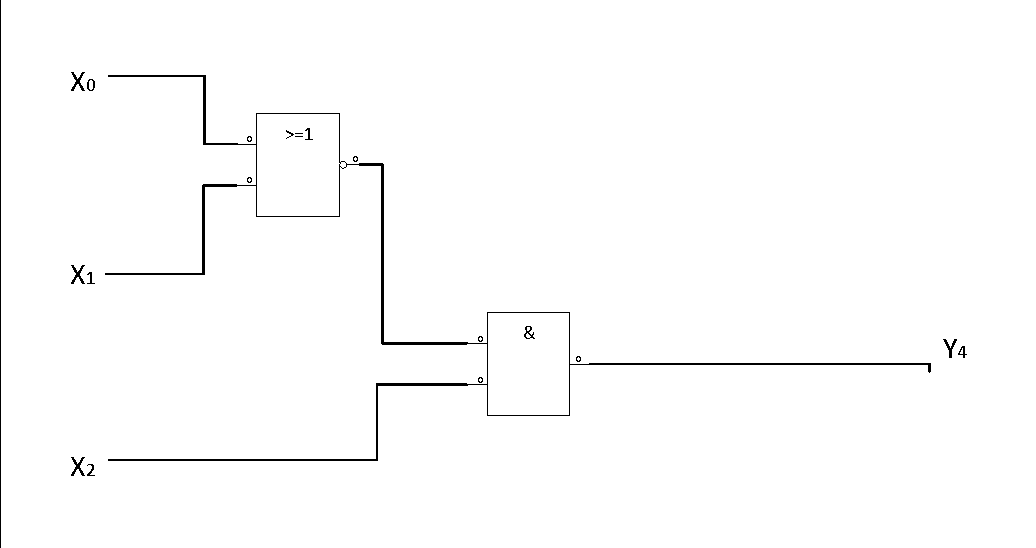
\includegraphics[width=10cm]{y4}\\
		y_5 = x_0\n{x_1}x_2\\
		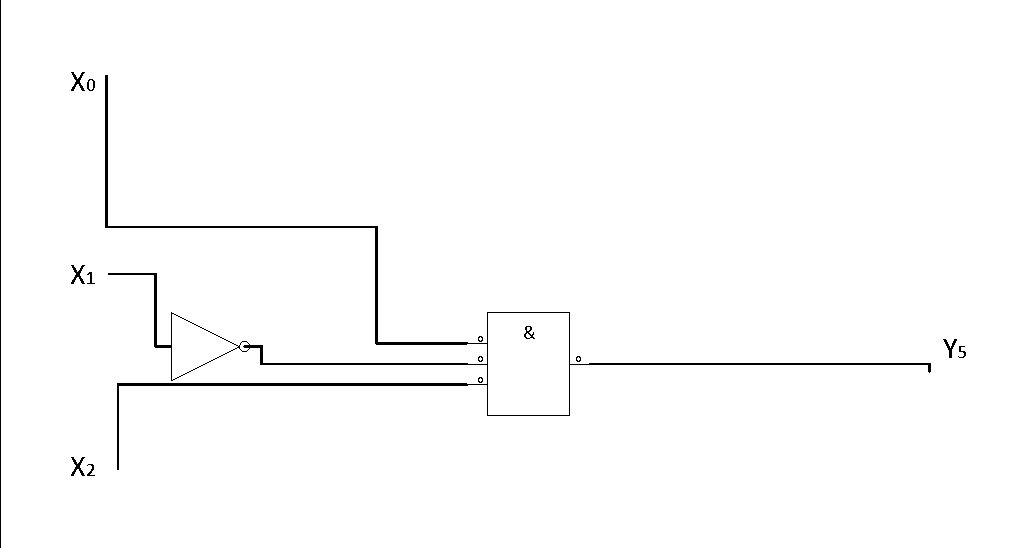
\includegraphics[width=10cm]{y5}\\
		y_6 = \n{x_0}x_1x_2\\
		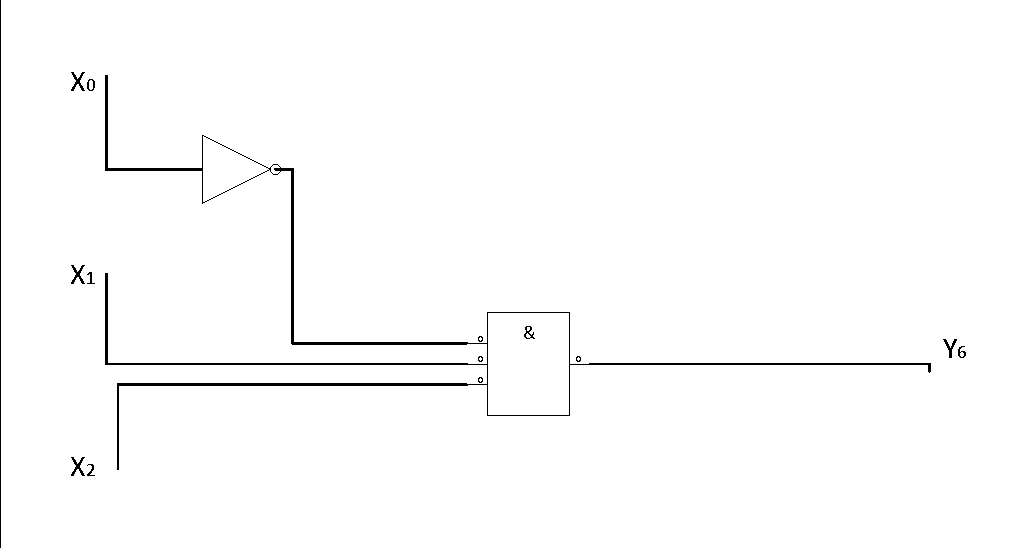
\includegraphics[width=10cm]{y6}\\
		y_7 = x_0x_1x_2\\
		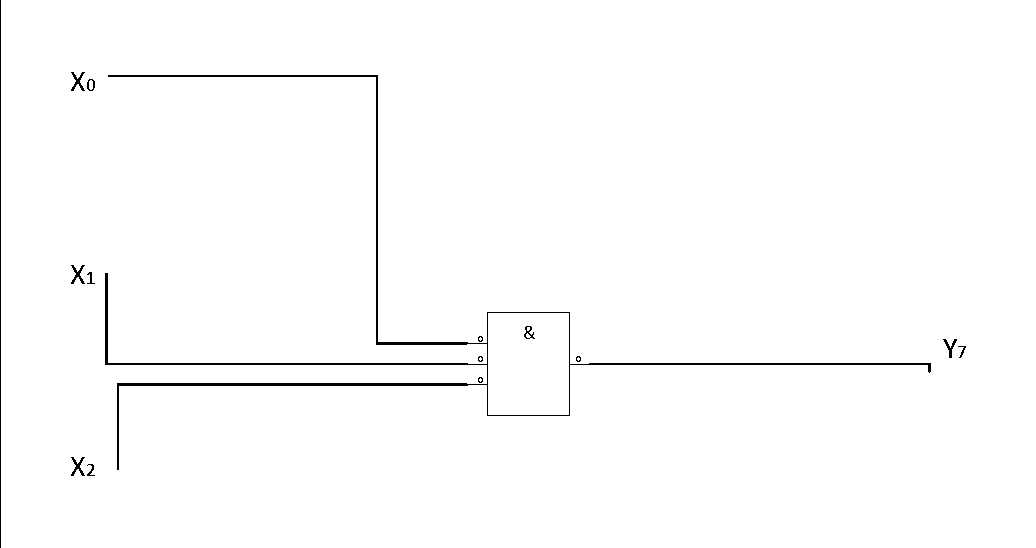
\includegraphics[width=10cm]{y7}\\
		\end{math}
		\end{description}
	\item[2.]
		\begin{description}
			\item[a)]
			\begin{tabular}{ c c c | c c c}
				$x_2$ & $x_1$ & $x_0$ & $y_2$
				& $y_1$ & $y_0$\\\hline
				0 & 0 & 0 & 0 & 0 & 0\\
				0 & 0 & 1 & 0 & 0 & 1\\
				0 & 1 & 0 & 0 & 1 & 1\\
				0 & 1 & 1 & 0 & 1 & 0\\
				1 & 0 & 0 & 1 & 1 & 0\\
				1 & 0 & 1 & 1 & 1 & 1\\
				1 & 1 & 0 & 1 & 1 & 1\\
				1 & 1 & 1 & 1 & 0 & 0\\
			\end{tabular}\\
		\end{description}
	\item[3.]
		\begin{description}
			\item[a)]
			\begin{tabular}{c | c  c c c | c c c c}
				$d$ & $x_3$ & $x_2$ & $x_1$ & $x_0$ & $y_3$ & $y_2$
				& $y_1$ & $y_0$\\\hline
				0 & 0 & 0 & 0 & 0 & 0 & 0 & 0 & 0\\
				1 & 0 & 0 & 0 & 1 & 0 & 0 & 0 & 1\\
				2 & 0 & 0 & 1 & 0 & 0 & 0 & 1 & 0\\
				3 & 0 & 0 & 1 & 1 & 0 & 0 & 1 & 1\\
				4 & 0 & 1 & 0 & 0 & 0 & 1 & 0 & 0\\
				5 & 0 & 1 & 0 & 1 & 1 & 0 & 1 & 1\\
				6 & 0 & 1 & 1 & 0 & 1 & 1 & 0 & 0\\
				7 & 0 & 1 & 1 & 1 & 1 & 1 & 0 & 1\\
				8 & 1 & 0 & 0 & 0 & 1 & 1 & 1 & 0\\
				9 & 1 & 0 & 0 & 1 & 1 & 1 & 1 & 1\\
			\end{tabular}\\
		Für die Darstellung von Zahlen größer als neun werden acht Bit benötigt.
		\item[b)]
		\begin{math}
		y_0 = x_0\n{x_1}\n{x_2}\n{x_3} + x_0x_1\n{x_2}\n{x_3} + x_0\n{x_1}x_2\n{x_3} + x_0x_1x_2\n{x_3} + x_0\n{x_1}\n{x_2}x_3\\
		y_1 = \n{x_0}x_1\n{x_2}\n{x_3} + x_0x_1\n{x_2}\n{x_3} + x_0\n{x_1}x_2\n{x_3} + \n{x_0}\n{x_1}\n{x_2}x_3 + x_0\n{x_1}\n{x_2}x_3\\
		y_2 =  \n{x_0}\n{x_1}x_2\n{x_3} + \n{x_0}x_1x_2\n{x_3} + x_0x_1x_2\n{x_3} + \n{x_0}\n{x_1}\n{x_2}x_3 + x_0\n{x_1}\n{x_2}x_3\\
		y_3 = x_0\n{x_1}x_2\n{x_3} + \n{x_0}x_1x_2\n{x_3} + x_0x_1x_2\n{x_3} + \n{x_0}\n{x_1}\n{x_2}x_3 + x_0\n{x_1}\n{x_2}x_3
		\end{math}
		\item[c)]
		\begin{math}
		y_0 = x_0\\\\
		\begin{tabular}{c | c | c | c | c | c}
			 & \n{x_0} & x_0 & x_0 & \n{x_0} & \\\hline
			\n{x_1} & 0 & 0 & 1 & 0 & \n{x_3}\\\hline 
			x_1 & 1 & 1 & 0 & 0 & \n{x_3}\\\hline
			x_1 & 1 & 1 & 1 & 1 & x_3\\\hline
			\n{x_1} & 1 & 1 & 1 & 1 & x_3\\\hline   
			& \n{x_2} & \n{x_2} & x_2 & x_2 & \\
		\end{tabular}\\
		\implies
		y_1 = x_1\n{x_2}\n{x_3} + x_0\n{x_1}x_2 + x_3\\\\
		\begin{tabular}{c | c | c | c | c | c}
			& \n{x_0} & x_0 & x_0 & \n{x_0} & \\\hline
			\n{x_1} & 0 & 0 & 0 & 0 & \n{x_3}\\\hline 
			x_1 & 1 & 0 & 1 & 1 & \n{x_3}\\\hline
			x_1 & 1 & 1 & 1 & 1 & x_3\\\hline
			\n{x_1} & 1 & 1 & 1 & 1 & x_3\\\hline   
			& \n{x_2} & \n{x_2} & x_2 & x_2 & \\
		\end{tabular}\\
		\implies
		y_2 = \n{x_0}x_1\n{x_3} + x_1x_2\n{x_3} + x_3\\\\
		\begin{tabular}{c | c | c | c | c | c}
			& \n{x_0} & x_0 & x_0 & \n{x_0} & \\\hline
			\n{x_1} & 0 & 0 & 1 & 1 & \n{x_3}\\\hline 
			x_1 & 1 & 0 & 1 & 1 & \n{x_3}\\\hline
			x_1 & 1 & 1 & 1 & 1 & x_3\\\hline
			\n{x_1} & 1 & 1 & 1 & 1 & x_3\\\hline   
			& \n{x_2} & \n{x_2} & x_2 & x_2 & \\
		\end{tabular}\\
		\implies
		y_3 = \n{x_0}x_1\n{x_3} + x_2 + x_3
		\end{math}
		\end{description}
	\end{description}
\end{document}